\documentclass{article}
\usepackage[utf8]{inputenc}
\usepackage{amsfonts}
\usepackage{amsmath}
\usepackage{graphicx}
\usepackage[a4paper, total={6in, 8in}]{geometry}
\usepackage{setspace}

\newcommand\tab[1][1cm]{\hspace*{#1}}
\onehalfspacing
\author{Frederic Becerril}

\begin{document}

\part*{Chapitre 3: Matrices et orthogonalité}

On se place ici dans un espace euclidien de dimension n.

\section{Écriture dans une base orthonormée.}

\subsection{\underline{Rappel:}}
Soit $\cal{E}$ une BON $\{e_1, \dots, e_n\}$ de E.\\
Comme c'est une base on peut à tout vecteur $\vec{x}$ de E associer ses coordonnées X $= \begin{pmatrix}
    x_1\\
    \vdots\\
    x_n\\
\end{pmatrix}$ dans la base $\cal{E}$ : $x = \sum x_i e_i$\\
Et on a un isomorphisme $\varphi_{\cal{E}} : E \rightarrow \mathbb{R}^n$\\
$\tab[4.7cm] x \longmapsto \begin{pmatrix}
    x_1\\
    \vdots\\
    x_n\\
\end{pmatrix} = X$

Mais comme la base est orthonormée, on connait facilement les coordonnées:

$$x = \sum_{i = 1}^n x_i e_i = \sum_{i = 1}^n <x | e_i> e_i \mbox{ ou encore } X = \begin{pmatrix}
    <x | e_i>\\
    \vdots\\
    <x | e_n>\\
\end{pmatrix}$$

Et dans ces conditions:
\begin{itemize}
    \item $<x | y> = \sum_{i = 1}^n x_i y_i = X^T . Y = \begin{pmatrix}
        x_1,
        \dots,
        x_n
    \end{pmatrix}
    \begin{pmatrix}
        y_1\\
        \vdots\\
        y_n\\
    \end{pmatrix}$
    \item $||x||^2 = \sum_{i = 1}^n x_i^2 = X^T . X = \sum_{i = 1}^n <x | e_i>^2$
\end{itemize}

Comme déjà vu, l'écriture dans une BON est facile à obtenir et pour ces coordonnées le produit scalaire usuel $\mathbb{R}^n$ qui fait intervenir la \underline{transposition}.




\subsection{\underline{Orthogonal et transposition}}

Soit $A \in M_{n, p}(\mathbb{R}) \tab A = \underset{\underset{1 \leq j \leq p}{1 \leq i \leq n}}{((a_{ij}))}$
Donc A $\begin{pmatrix}
    a_{11} & \dots & a_{ip}\\
    \vdots & & \vdots\\
    a_{n1} & \dots & a_{np}\\
\end{pmatrix}$, on rappelle que :\\
$ker A = \left\{ X = \begin{pmatrix}
    x_1\\
    \vdots\\
    x_p\\
\end{pmatrix} \mbox{ tq } AX = \begin{pmatrix}
    0\\
    \vdots\\
    0\\
\end{pmatrix} \right\}$\\
$ImA = \left\{AX \;;\; x \in \mathbb{R}^p
\right\}$.
\paragraph{\underline{Proposition}} Soit $\{f_1, \dots, f_p\}$ p vecteurs de E\\
et A la matrice constituée des vecteurs colonnes de $f_1, \dots, f_p$ dans une BON de \cal{E}. i.e $A = Mat_{\cal{E}}(f_1, \dots, f_p)$\\
Dans la base $\cal{E}$ : $Vect\{f_1, \dots, f_p\}^\perp = ker(A^T)$\\

Ceci veut dire que $x \in Vect\{f_1, \dots, f_p\}^\perp$ SSI ses coordonnées X sont dans $ker(A^T)$

\paragraph{\underline{Preuve:}}

Ici $A = ((a_{ij}))$\\ 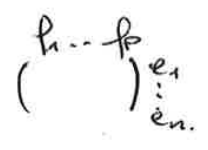
\includegraphics{images/image01.png}\\
Donc $\forall 1 \leq j \leq n \tab[0.5cm] f_j = \sum_{i =1}^n a_{ij} e_i \mbox{ on note } A_j = \begin{pmatrix}
    a_{1j}\\
    \vdots\\
    a_{nj}\\
\end{pmatrix}$\\
Si $W = Vect\{f_1, \dots, f_p\}$,
\begin{itemize}
    \item[$x \in W^\perp$] $\Leftrightarrow \forall 1 \leq j \leq p \tab[0.5cm] <f_j | x> = 0$
    \item[] $x \rightarrow \sum x_i e_i x \begin{pmatrix}
        x_1\\
        \vdots\\
        x_n\\
    \end{pmatrix}$
    \item[] $\Leftrightarrow \forall 1 \leq j \leq p \tab[0.5cm] A_j^T . X = 0$
    \item[] $\Leftrightarrow \begin{pmatrix}
        A_1^T . X\\
        \vdots\\
        A_p^T . X
    \end{pmatrix} = \begin{pmatrix}
        0\\
        \vdots\\
        0\\
    \end{pmatrix}_p$
    \item[Mais ici] $A_j^T X = \sum_{i = 1}^n a_{ij} x_i \tab[0.5cm] \mbox{ et si } B = A^T alors b_{ji} = a{ij}$
    \item[] $A_j^T X = \sum b_{ji} x_i$
    \item[donc $x \in W^\perp$] $\Leftrightarrow \begin{pmatrix}
        A_1^T\\
        \dots\\
        \dots\\
        A_p^T
    \end{pmatrix} \circ \begin{pmatrix}
        x_1\\
        \vdots\\
        x_n\\
    \end{pmatrix} = 0$
    \item[] $\Leftrightarrow A^T \circ \begin{pmatrix}
        x_1\\
        \vdots\\
        x_n\\
    \end{pmatrix} = 0$
    \item[] $\Leftrightarrow \begin{pmatrix}
        x_1\\
        \vdots\\
        x_n\\
    \end{pmatrix} \in ker A^T$
\end{itemize}
On voit ici que dans une BON, l'orthogonalité est liée à la transposition des matrices.\\
Par ailleurs, cette proposition n'est pas sans rappeler. les matrices de changements de base.\\

\subsection{\underline{Rappel sur les changements de base}}
Si $\cal{E}$ = $\{e_1, \dots, e_n\}$ et $\cal{F}$ = $\{f_1, \dots, f_n\}$ sont des bases d'un ev E de dimension n.\\
On appelle la matrice de passage $\mathcal E \mbox{ à } \mathcal{F}$ la matrice $P \in M_n(\mathbb{R}) \tab P = mat_{\mathcal{E}}(f_1 \; \dots \; f_n)$\\
Si $P = ((p_{ij}))_{1 \leq i,j \leq n} \tab f_j = \sum_{i = 1}^n p_{ij} e_i$\\
On rappelle que si x a pour coordonnées $X = \begin{pmatrix}
    x_1\\
    \vdots\\
    x_n\\
\end{pmatrix}$ dans $\mathcal{E}$ et $X' = \begin{pmatrix}
    x'_1\\
    \vdots\\
    x'_n
\end{pmatrix}$ dans $\mathcal{F}$ alors:

\begin{align*}
    \fbox{X = PX'}
\end{align*}
De plus si v est un endomorphisme de E de matrice représentative A dans $\mathcal{E}$ et A' dans $\mathcal{F}$ alors
\begin{align*}
    \fbox{$A' = P^{-1} A P$}
\end{align*}
Que se passe-t-il avec des BON

\section{BON et Matrices orthogonalles.}

\subsection{\underline{Résultat préliminaire:}}
Soit $\cal E$ une BON de E et $\{f_1, \dots, f_p\}$ p vecteurs de E\\
De nouveau on pase $A = Mat_{\mathcal{E}}(f_1, \dots, f_p) \in M_{n, p}(\mathbb{R})$\\
Si M est la matrice $p \times p$ constituée des produit scalaires $<f_i | f_j>$ alors\\

$M = A^T . A = \begin{pmatrix}
    <f_1 | f_1> & \dots & <f_1 | f_p>\\
    \vdots & & \vdots\\
    <f_p | f_1> & \dots & <f_p | f_p>\\
\end{pmatrix}$\\
Si $A = \begin{pmatrix}
    a_{1,1} & \dots & a_{1,p}\\
    \vdots & & \vdots\\
    a_{n,1} & \dots & a_{n,p}\\ 
\end{pmatrix} \tab[0.5cm] B = A^T = \begin{pmatrix}
    b_{1,1} & \dots & b_{1,n}\\
    \vdots & & \vdots\\
    b_{p,1} & \dots & b_{p,n}\\ 
\end{pmatrix} = \begin{pmatrix}
    a_{1,1} & a_{2, 1} & \dots & a_{n,1}\\
    \vdots & \vdots & & \vdots\\
    a_{1,p} & a_{2, p} & \dots & a_{n,p}\\ 
\end{pmatrix}$
$b_{i,j} = a_{j,i}$\\
d'un côté:\\
$<f_i | f_j>$ = $\left<\sum_{k = 1}^n a_{k, i} e_k \; , \; \sum_{l = 1}^n a_{l, j} e_j
\right>$\\
$\tab[1.56cm] = \sum_{k=1}^n a_{k, i} a_{l, j} <e_k | e_l>$\\
$\tab[1.56cm] = \sum_{k=1}^n a_{k, i} a_{k, j}$\\
Si $M = A^T A =$



\end{document}